\documentclass[10pt,a4paper]{article}

\usepackage[utf8]{inputenc}
\usepackage[T1]{fontenc}
\usepackage[brazil]{babel}
\usepackage{lmodern}
\usepackage{geometry}
\geometry{
	top=1.2cm,
	bottom=1.3cm,
	left=1.5cm,
	right=1.5cm
}

\usepackage{xcolor}
% Paleta Institucional
\definecolor{bisnavy}{RGB}{14, 30, 54}
\definecolor{bisblue}{RGB}{28, 64, 105}
\definecolor{bistile}{RGB}{60, 100, 145}
\definecolor{bisterra}{RGB}{192, 75, 55}
\definecolor{bisgold}{RGB}{220, 150, 60}
\definecolor{bislight}{RGB}{240, 244, 250}
\definecolor{secondary}{RGB}{90, 100, 110}
\definecolor{rulecolor}{RGB}{215, 220, 225}
\definecolor{boxbg}{RGB}{248, 250, 252}

% Cores do Quote e Resumo Executivo
\definecolor{corFundoQuote}{RGB}{244, 247, 253}
\definecolor{corBarraQuote}{RGB}{28, 64, 105}
\definecolor{corAzulExecutivo}{RGB}{248, 251, 255}
\definecolor{corBordaExecutivo}{RGB}{215, 228, 245}

\usepackage{tikz}
\usetikzlibrary{shapes,positioning,calc}

\usepackage{graphicx}
\usepackage{booktabs}
\usepackage{enumitem}
\usepackage{caption}
\captionsetup{
	position=top,
	skip=3pt,
	labelfont={bf,footnotesize,color=bisnavy},
	textfont={footnotesize,color=bisnavy}
}

\usepackage{tcolorbox}
\tcbuselibrary{skins,breakable}

\usepackage{siunitx}
\sisetup{output-decimal-marker={,}}

\usepackage{hyperref}
\hypersetup{
	colorlinks=true,
	linkcolor=bisblue,
	urlcolor=bisblue,
	citecolor=bisblue
}

\tcbset{
	quotebox/.style={
		enhanced,
		colback=corFundoQuote,
		boxrule=0pt,
		frame hidden,
		borderline west={2.5pt}{0pt}{corBarraQuote},
		arc=0pt,
		left=10pt,
		right=10pt,
		top=6pt,
		bottom=6pt
	},
	resumobox/.style={
		colback=corAzulExecutivo,
		colframe=corBordaExecutivo,
		boxrule=0.5pt,
		arc=2.5pt,
		left=8pt,
		right=8pt,
		top=5pt,
		bottom=5pt
	},
	notabox/.style={
		colback=white,
		colframe=rulecolor,
		boxrule=0.6pt,
		arc=2pt,
		left=8pt,
		right=8pt,
		top=5pt,
		bottom=5pt
	},
	downloadbox/.style={
		colback=white,
		colframe=bistile!60,
		boxrule=0.6pt,
		arc=2pt,
		left=8pt,
		right=8pt,
		top=5pt,
		bottom=5pt
	}
}

\setlength{\parindent}{0pt}
\setlength{\parskip}{3.5pt}

% Comando único de cabeçalho
\newcommand{\cabecalhopadrao}{
	\noindent
	{\large \bfseries \color{bisnavy} Monitor da Inflação Alimentar}
	\vspace{3pt}
	\noindent
	{\footnotesize \color{secondary} Itaiguara de Oliveira Bezerra \quad\textbar\quad Economista Sênior e de Dados \quad\textbar\quad {\bfseries\color{bisblue}Por Estrato de Renda -- Outubro de 2026}}
	\vspace{1.5pt}
	\noindent
	{\footnotesize \color{secondary} \texttt{itaiguara-bezerra.github.io}}
	\vspace{0.10cm}
	{\color{rulecolor}\hrule height 0.6pt}
	\vspace{0.20cm}
}

\begin{document}
	
	% ==============================================================================
	% CAPA EDITORIAL (NÃO CONTADA NA NUMERAÇÃO DE PÁGINAS)
	% ==============================================================================
	\begin{titlepage}
		\newgeometry{top=0cm, bottom=0cm, left=0cm, right=0cm}
		\noindent
		\begin{tikzpicture}[x=1cm, y=1cm]
			\path (0,0) rectangle (21, 29.7);
			
			\fill[bisnavy] (0, 29.7) -- (21, 29.7) -- (21, 16.5) -- (0, 12.0) -- cycle;
			\fill[bisblue] (0, 12.0) -- (21, 16.5) -- (21, 14.8) -- (0, 10.3) -- cycle;
			\fill[bistile] (0, 10.3) -- (21, 14.8) -- (21, 13.8) -- (0, 9.3) -- cycle;
			\fill[bisterra] (0, 9.3) -- (21, 13.8) -- (21, 12.8) -- (0, 8.3) -- cycle;
			\fill[bisgold] (0, 8.3) -- (21, 12.8) -- (21, 12.3) -- (0, 7.8) -- cycle;
			
			\fill[bislight] (0, 2.2) -- (21, 2.2) -- (21, 11.0) -- (0, 6.5) -- cycle;
			\fill[bistile, opacity=0.15] (5, 2.2) -- (21, 9.5) -- (21, 2.2) -- cycle;
			\fill[bisnavy, opacity=0.08] (0, 2.2) -- (14, 2.2) -- (0, 7.0) -- cycle;
			
			\fill[bisnavy] (0, 0) rectangle (21, 2.2);
			\fill[bisterra] (0, 2.2) rectangle (21, 2.4);
			
			\draw[white, opacity=0.3, line width=1.2pt] (1.8, 17.0) -- (19.2, 21.0);
			\draw[bisgold, opacity=0.6, line width=0.8pt] (1.8, 16.5) -- (19.2, 20.5);
			
			\node[anchor=north west, text=white, opacity=0.80, font=\scriptsize\sffamily\bfseries] 
			at (1.8, 28.0) {RELATÓRIO DE MONITORAMENTO MACROECONÔMICO};
			
			\node[anchor=north west, text=white, font=\huge\sffamily\bfseries, text width=17.5cm, align=left] 
			at (1.8, 26.5) {Monitor da Inflação Alimentar};
			
			\node[anchor=north west, text=bisgold, font=\Large\sffamily\bfseries] 
			at (1.8, 23.2) {Por Estrato de Renda -- Outubro de 2026};
			
			\node[anchor=north, text=white, font=\Large\sffamily\itshape, text width=17.5cm, align=center] 
			at (10.5, 21.4) {A dinâmica dos preços alimentares nos diferentes estratos de renda familiar};
			
			\node[anchor=south east, align=right] at (19.2, 3.2) {
				\color{bisnavy}\bfseries\large Itaiguara de Oliveira Bezerra\\[3pt]
				\color{secondary}\footnotesize Economista Sênior e de Dados\\[2pt]
				\color{secondary}\footnotesize Pesquisador Independente\\[2pt]
				\color{bistile}\footnotesize \texttt{itaiguara@terra.com.br}\\[2pt]
				\color{bisnavy}\footnotesize \texttt{itaiguara-bezerra.github.io}\\[5pt]
				\color{black}\scriptsize\bfseries Divulgado em 12 de novembro de 2026.
			};
			
			\node[anchor=west, text=white, opacity=0.85, font=\scriptsize\sffamily] 
			at (1.8, 1.1) {Pesquisa Econômica Independente \quad\textbar\quad Metodologia POF / IBGE};
			
			\node[anchor=east, text=white, font=\scriptsize\sffamily\bfseries] 
			at (19.2, 1.1) {Série Histórica e Monitoramento Mensal};
		\end{tikzpicture}
	\end{titlepage}
	\restoregeometry
	
	% ==============================================================================
	% PÁGINA 1: INDICADORES, PANORAMA, FIGURA 1 E TABELA 1
	% ==============================================================================
	\cabecalhopadrao
	
	\noindent
	\begin{minipage}[t]{0.24\textwidth}
		\centering
		{\footnotesize \bfseries IPCA GERAL}\\[1.5pt]
		{\large \bfseries \color{bisterra} +0,14\%}\\[1pt]
		{\scriptsize Variação mensal}
	\end{minipage}
	\hfill
	\begin{minipage}[t]{0.24\textwidth}
		\centering
		{\footnotesize \bfseries IPCA -- DOMICÍLIO}\\[1.5pt]
		{\large \bfseries \color{bisterra} +1,31\%}\\[1pt]
		{\scriptsize Variação mensal}
	\end{minipage}
	\hfill
	\begin{minipage}[t]{0.24\textwidth}
		\centering
		{\footnotesize \bfseries RENDA MUITO BAIXA}\\[1.5pt]
		{\large \bfseries \color{bisterra} +0,64\%}\\[1pt]
		{\scriptsize Menor rendimento}
	\end{minipage}
	\hfill
	\begin{minipage}[t]{0.24\textwidth}
		\centering
		{\footnotesize \bfseries RENDA ALTA}\\[1.5pt]
		{\large \bfseries \color{bisterra} +0,72\%}\\[1pt]
		{\scriptsize Maior rendimento}
	\end{minipage}
	
	\vspace{0.15cm}
	{\color{rulecolor}\hrule height 0.6pt}
	\vspace{0.15cm}
	
	\begin{tcolorbox}[quotebox]
		\small\itshape
		``Em outubro, apesar de se manterem em patamar elevado, as taxas de inflação da alimentação no domicílio arrefeceram na maioria das faixas de renda, com exceção da Renda Média-Baixa (que acelerou 0,23 p.p.). A variação foi de +0,64\% na Renda Muito Baixa e de +0,72\% na Renda Alta. A Renda Média registrou a maior taxa mensal (+0,83\%), situando-se acima do IPCA Geral (+0,14\%), porém abaixo do IPCA de Alimentação no Domicílio (+1,31\%).''
		\vspace{3pt}
		\par\raggedleft\normalfont\footnotesize --- Itaiguara Bezerra, Economista Sênior e de Dados
	\end{tcolorbox}
	
	\vspace{0.10cm}
	
	\begin{tcolorbox}[resumobox]
		\noindent {\bfseries\normalsize \color{bisnavy} Resumo Executivo:}
		\begin{itemize}[leftmargin=12pt, itemsep=2pt, topsep=2pt, parsep=0pt]
			
			\item {\small Diferenças de intensidade: a Renda Muito Baixa registrou variação de +0,64\%, enquanto a Renda Alta anotou +0,72\% (diferença estreita de 0,08 p.p. entre os extremos).}
			
			\item {\small Referência oficial: o IPCA de Alimentação no Domicílio registrou alta de +1,31\%, descolando-se significativamente da maior variação por estrato (Renda Média, +0,83\%).}
			
			\item {\small Pressão generalizada: todos os grupos de consumo apresentaram alta. O destaque foi Proteínas Animais, que afetou todas as faixas e exerceu maior impacto na Renda Média-Baixa (+0,33 p.p.) e Renda Muito Baixa (+0,29 p.p.).}
			
			\item {\small Vetor secundário: o grupo Frutas e Hortaliças também exerceu forte influência altista, de forma mais concentrada a partir da Renda Média-Baixa.}
			
		\end{itemize}
	\end{tcolorbox}
	
	\vspace{0.12cm}
	
	\noindent {\large \bfseries \color{bisnavy} Panorama do Mês e Trajetória Recente}
	
	\vspace{0.06cm}
	
	{\small Apesar da perda de fôlego na margem, todas as faixas de renda registraram inflação positiva em outubro (com a Renda Média-Baixa indo na contramão e acelerando no mês). Conforme ilustra o painel à direita, a Renda Média registrou a maior alta (0,83\%), seguida pela Renda Média-Baixa (0,80\%) e Renda Média-Alta (0,74\%). A trajetória semestral — ilustrada no gráfico à esquerda — mantém viés de alta estrutural, a despeito do alívio pontual no mês.}
	
	\vspace{0.06cm}
	
	\begin{figure}[h!]
		\centering
		\caption{Trajetória semestral e variação no mês: Estratos de Renda vs. IPCA Alimentação no Domicílio.}
		\vspace{2pt}
		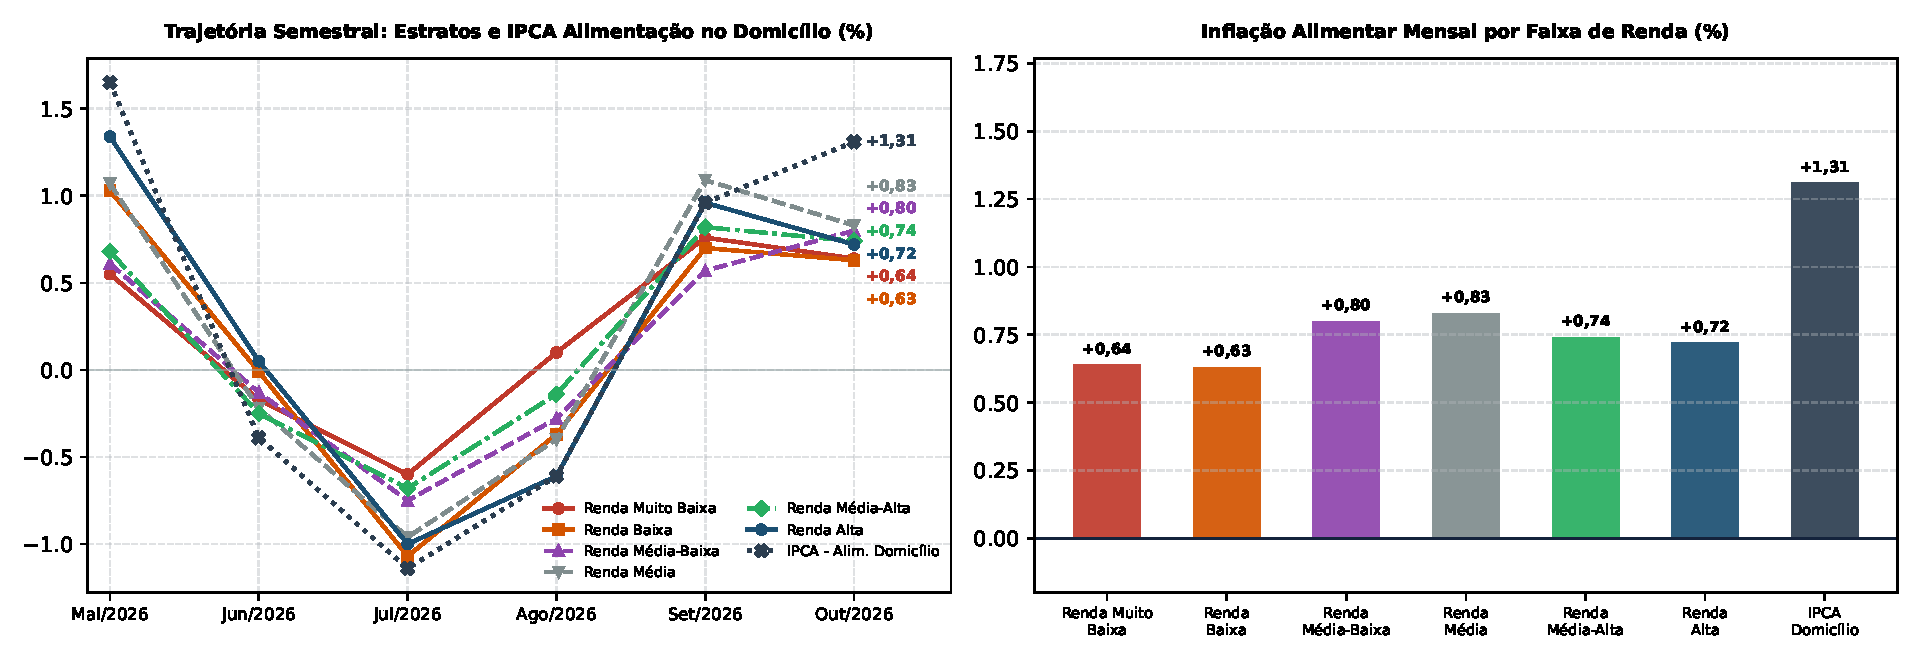
\includegraphics[width=\textwidth]{painel_1x2_trajetoria_barras.pdf}
		\vspace{2pt}
		\noindent\raggedright
		{\tiny \color{secondary} Fonte: Elaboração do autor com base em dados da POF 2017--2018 e Tabela 7060 (SIDRA/IBGE).}
	\end{figure}
	
	\vspace{0.15cm}
	
	\begin{table}[h!]
		\centering
		\caption{Variação Mensal e Acumulada (\%)}
		\vspace{1pt}
		\footnotesize
		\begin{tabular*}{\textwidth}{@{\extracolsep{\fill}} l c c c c c @{}}
			\toprule
			& \multicolumn{3}{c}{\textbf{Variação Mensal}} & \multicolumn{2}{c}{\textbf{Variação Acumulada}} \\
			\cmidrule(lr){2-4} \cmidrule(lr){5-6}
			\textbf{Estrato / Indicador} & \textbf{Ago./26} & \textbf{Set./26} & \textbf{Out./26} & \textbf{12 Meses} & \textbf{No Ano} \\
			\midrule
			IPCA Geral & -0,32 & 0,82 & 0,14 & 4,63 & 4,10 \\
			IPCA - Alim. Domicílio & -0,61 & 0,96 & 1,31 & 5,72 & 5,78 \\
			\midrule
			
			Renda Muito Baixa & 0,10 & 0,76 & 0,64 & 6,20 & 5,33 \\
			
			Renda Baixa & -0,37 & 0,70 & 0,63 & 6,91 & 6,16 \\
			
			Renda Média-Baixa & -0,28 & 0,57 & 0,80 & 6,08 & 5,06 \\
			
			Renda Média & -0,40 & 1,09 & 0,83 & 7,34 & 6,18 \\
			
			Renda Média-Alta & -0,14 & 0,82 & 0,74 & 6,03 & 5,24 \\
			
			Renda Alta & -0,61 & 0,96 & 0,72 & 6,91 & 6,05 \\
			
			\bottomrule
		\end{tabular*}
	\end{table}
	
	\clearpage
	
	% ==============================================================================
	% PÁGINA 2: TENDÊNCIA E DECOMPOSIÇÃO
	% ==============================================================================
	\cabecalhopadrao
	
	\noindent {\large \bfseries \color{bisnavy} Análise de Tendência e Suavização}
	
	\vspace{0.06cm}
	
	{\small A comparação entre a tendência anualizada e a medida suavizada (EWMA) permite avaliar se a inflação alimentar está ganhando ou perdendo intensidade. Valores da tendência anualizada superiores ao EWMA sugerem aceleração recente dos preços, enquanto valores inferiores indicam arrefecimento. O descolamento entre a tendência anualizada e a medida suavizada foi mais expressivo nas faixas Renda Média-Baixa e Renda Média, sinalizando pressões recentes mais intensas sobre a cesta destes estratos.}
	
	\vspace{0.25cm}
	
	\begin{table}[h!]
		\centering
		\caption{Tendências da Inflação Alimentar (\% ao ano)}
		\vspace{1pt}
		\footnotesize
		\begin{minipage}{0.80\textwidth}
			\begin{tabular*}{\linewidth}{@{\extracolsep{\fill}} l c c @{}}
				\toprule
				& \multicolumn{2}{c}{\textbf{Taxas Anualizadas (\% ao ano)}} \\
				\cmidrule(lr){2-3}
				\textbf{Faixa de Renda} & \begin{tabular}{@{}c@{}}\textbf{\color{bisnavy}Tendência} \\ \textbf{\color{bisnavy}(com base no resultado do mês)}\end{tabular} & \textbf{Suavização} \\
				\midrule
				
				Renda Muito Baixa & +7,96 & +4,90 \\
				
				Renda Baixa & +7,83 & +4,75 \\
				
				Renda Média-Baixa & +10,03 & +4,38 \\
				
				Renda Média & +10,43 & +5,53 \\
				
				Renda Média-Alta & +9,25 & +4,77 \\
				
				Renda Alta & +8,99 & +4,99 \\
				
				\bottomrule
			\end{tabular*}
			\vspace{4pt}\par
			\noindent
			{\tiny \color{secondary} \textbf{Nota Metodológica:} O método de suavização utilizado é a Média Móvel Exponencialmente Ponderada (EWMA). Para maiores detalhes sobre a modelagem, a Nota Técnica encontra-se disponível para \textit{download} na seção de \textbf{Repositório Público} (pág. 4).\par}
		\end{minipage}
	\end{table}
	
	\vspace{0.4cm}
	
	\noindent {\large \bfseries \color{bisnavy} O que Explicou a Variação Mensal}
	
	\vspace{0.06cm}
	
	{\small A decomposição das contribuições mostra que Proteínas Animais foi o grupo de maior impacto positivo em todos os estratos. Essa dinâmica reflete o forte aquecimento do setor no comércio externo, que exerce pressão direta sobre os preços internos. O grupo Frutas e Hortaliças atuou como o segundo vetor de alta, puxado sobretudo pelo tomate: temperaturas mais baixas comprometeram a maturação e restringiram a oferta do fruto no mercado.}
	
	\vspace{0.08cm}
	
	\begin{figure}[h!]
		\centering
		\caption{Contribuições dos grupos de produtos para a inflação mensal, por estrato de renda (p.p.)}
		\vspace{2pt}
		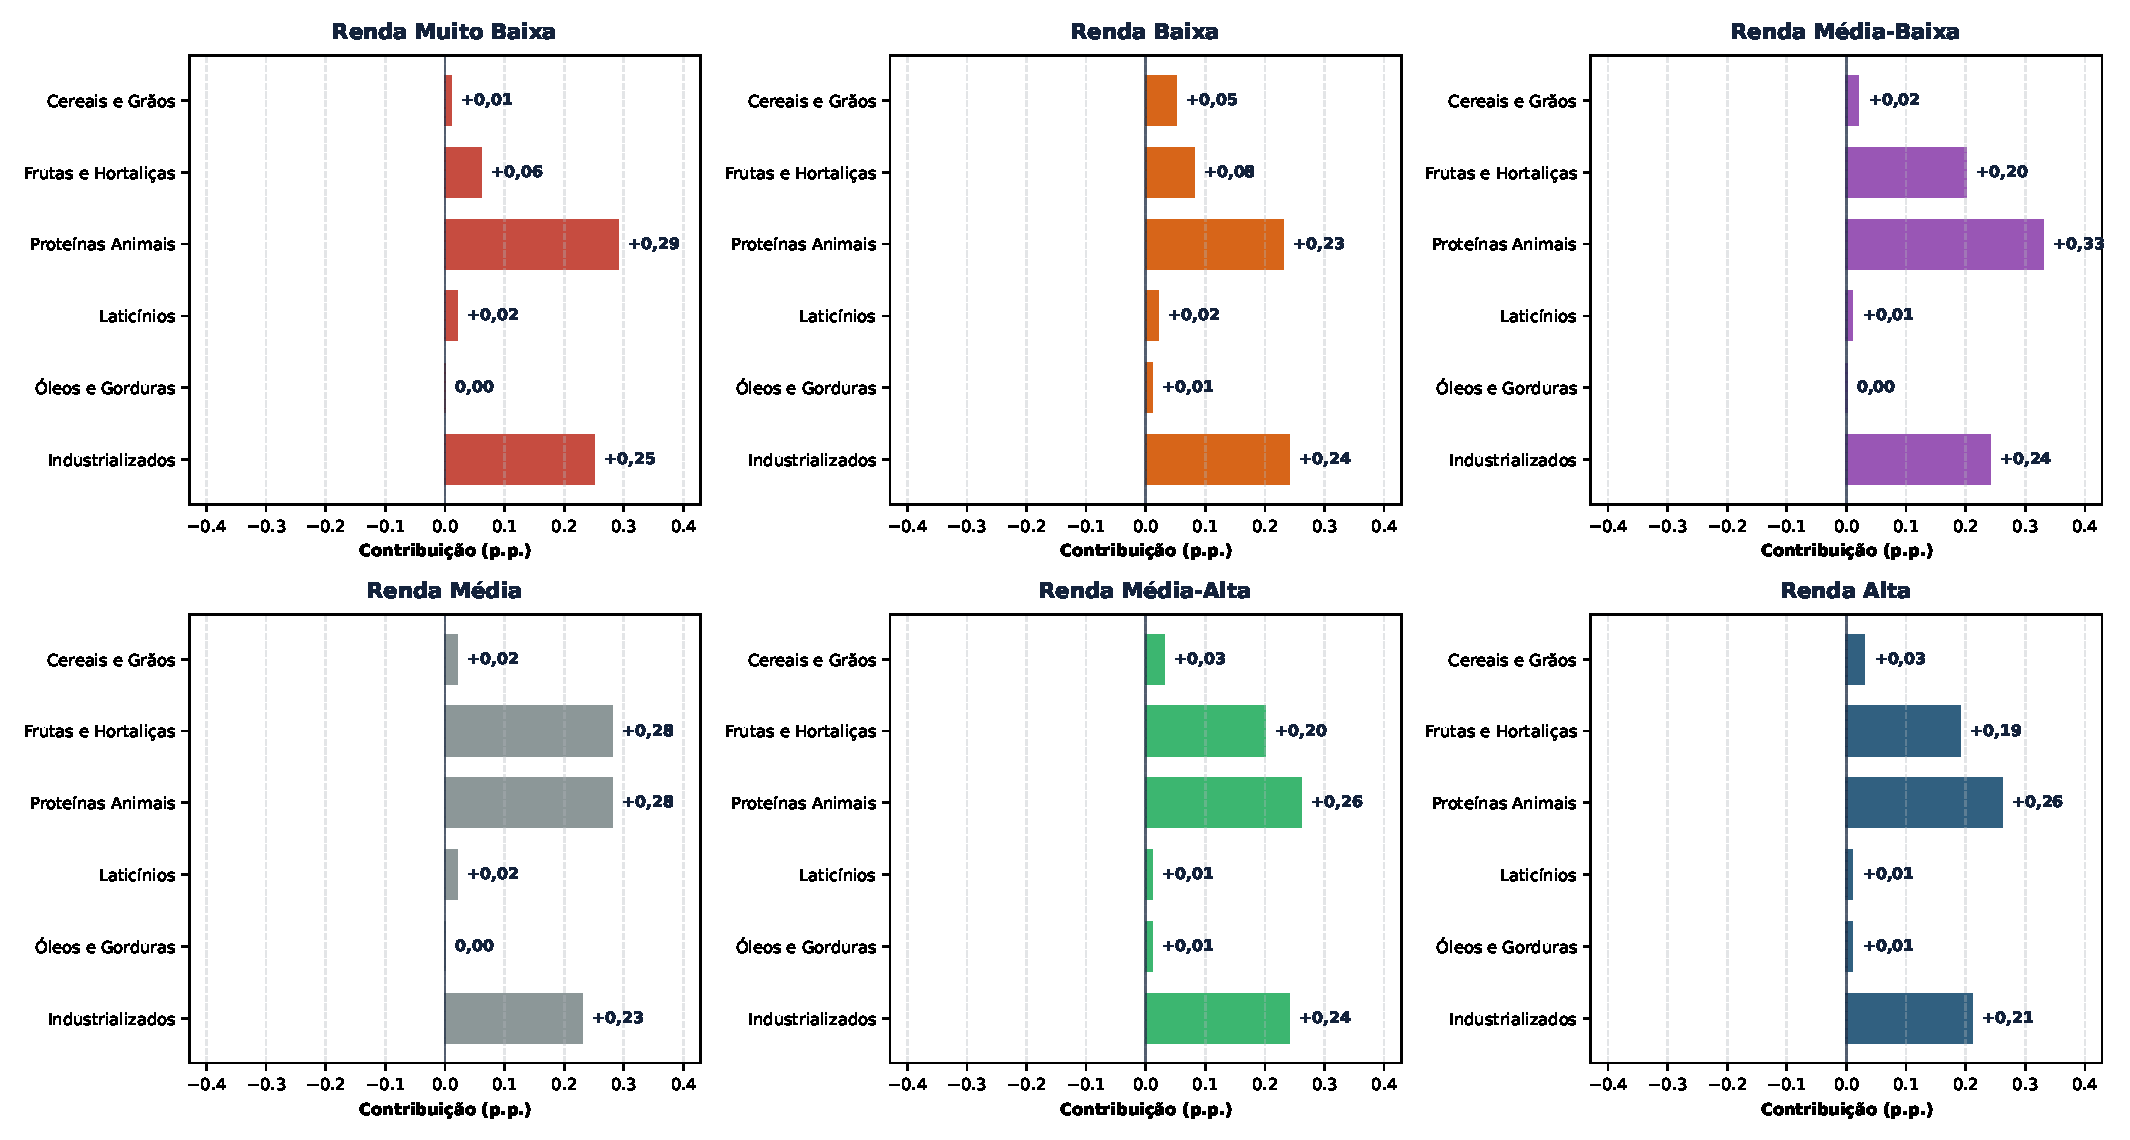
\includegraphics[width=\textwidth]{painel_contribuicao_6faixas.pdf}\par
		\vspace{4pt}
		\begin{flushleft}
			{\tiny \color{secondary} Fonte: Elaboração do autor com base em dados da POF 2017--2018 e Tabela 7060 (SIDRA/IBGE).\par}
		\end{flushleft}
	\end{figure}
	
	\clearpage
	
	% ==============================================================================
	% PÁGINA 3: TABELA 3 (SUBITENS)
	% ==============================================================================
	\cabecalhopadrao
	
	\noindent {\large \bfseries \color{bisnavy} Principais Contribuições Marginais de Subitens Alimentares por Estrato}
	\vspace{0.02cm}
	{\color{rulecolor}\hrule height 0.6pt}
	\vspace{0.06cm}
	
	{\small A tabela abaixo discrimina os cinco subitens que exerceram as maiores contribuições marginais positivas e negativas na formação da taxa mensal de cada estrato em Outubro de 2026.}
	
	\vspace{0.05cm}
	
	\begin{table}[h!]
		\centering
		\caption{Principais Contribuições Marginais de Subitens Alimentares por Estrato (Outubro de 2026)}
		\vspace{2pt}
		\footnotesize
		\renewcommand{\arraystretch}{1.15} % Aumenta o espaçamento vertical entre as linhas
		\setlength{\tabcolsep}{7pt} % Aumenta o respiro horizontal das colunas
		\begin{tabular*}{\textwidth}{@{\extracolsep{\fill}} c l c c | l c c @{}}
			\toprule
			& \multicolumn{3}{c}{\textbf{Maiores Altas (+) por Contribuição}} & \multicolumn{3}{c}{\textbf{Maiores Quedas (--) por Contribuição}} \\
			\cmidrule(lr){2-4} \cmidrule(lr){5-7}
			\textbf{\#} & \textbf{Alimento} & \textbf{Var. (\%)} & \textbf{Contrib. (p.p.)} & \textbf{Alimento} & \textbf{Var. (\%)} & \textbf{Contrib. (p.p.)} \\
			\midrule
			
			\multicolumn{7}{l}{\textbf{\color{bisnavy}Renda Muito Baixa}} \\
			\midrule
			
			1 & Tomate & +19,57 & +0,0619 & Manga & -12,27 & -0,1336 \\
			
			2 & Couve-flor & +5,82 & +0,0546 & Melão & -6,53 & -0,0666 \\
			
			3 & Cebola & +11,29 & +0,0517 & Cenoura & -9,72 & -0,0513 \\
			
			4 & Pimentão & +6,70 & +0,0506 & Feijão - mulatinho & -3,26 & -0,0349 \\
			
			5 & Coentro & +4,54 & +0,0486 & Melancia & -2,97 & -0,0315 \\
			
			\midrule
			
			\multicolumn{7}{l}{\textbf{\color{bisnavy}Renda Baixa}} \\
			\midrule
			
			1 & Tomate & +19,57 & +0,0931 & Cenoura & -9,72 & -0,0961 \\
			
			2 & Cheiro-verde & +5,45 & +0,0444 & Melão & -6,53 & -0,0489 \\
			
			3 & Coentro & +4,54 & +0,0439 & Manga & -12,27 & -0,0389 \\
			
			4 & Arroz & +4,81 & +0,0393 & Banana-da-terra & -2,78 & -0,0266 \\
			
			5 & Cebola & +11,29 & +0,0311 & Repolho & -5,34 & -0,0258 \\
			
			\midrule
			
			\multicolumn{7}{l}{\textbf{\color{bisnavy}Renda Média-Baixa}} \\
			\midrule
			
			1 & Cebola & +11,29 & +0,0707 & Cenoura & -9,72 & -0,0593 \\
			
			2 & Mamão & +6,43 & +0,0644 & Abobrinha & -4,83 & -0,0462 \\
			
			3 & Tomate & +19,57 & +0,0528 & Manga & -12,27 & -0,0440 \\
			
			4 & Coentro & +4,54 & +0,0434 & Abacaxi & -2,30 & -0,0237 \\
			
			5 & Cheiro-verde & +5,45 & +0,0416 & Peixe - cavala & -2,26 & -0,0226 \\
			
			\midrule
			
			\multicolumn{7}{l}{\textbf{\color{bisnavy}Renda Média}} \\
			\midrule
			
			1 & Tomate & +19,57 & +0,2040 & Cenoura & -9,72 & -0,0775 \\
			
			2 & Cebola & +11,29 & +0,1189 & Melão & -6,53 & -0,0587 \\
			
			3 & Couve-flor & +5,82 & +0,0585 & Manga & -12,27 & -0,0516 \\
			
			4 & Peixe - curimatã & +4,09 & +0,0401 & Repolho & -5,34 & -0,0505 \\
			
			5 & Mamão & +6,43 & +0,0351 & Feijão - mulatinho & -3,26 & -0,0338 \\
			
			\midrule
			
			\multicolumn{7}{l}{\textbf{\color{bisnavy}Renda Média-Alta}} \\
			\midrule
			
			1 & Tomate & +19,57 & +0,1017 & Manga & -12,27 & -0,0874 \\
			
			2 & Cebola & +11,29 & +0,0882 & Cenoura & -9,72 & -0,0692 \\
			
			3 & Couve-flor & +5,82 & +0,0589 & Peixe - aruanã & -3,33 & -0,0331 \\
			
			4 & Inhame & +6,46 & +0,0469 & Banana-da-terra & -2,78 & -0,0303 \\
			
			5 & Mamão & +6,43 & +0,0449 & Abobrinha & -4,83 & -0,0282 \\
			
			\midrule
			
			\multicolumn{7}{l}{\textbf{\color{bisnavy}Renda Alta}} \\
			\midrule
			
			1 & Tomate & +19,57 & +0,1439 & Manga & -12,27 & -0,0701 \\
			
			2 & Cebola & +11,29 & +0,0628 & Abobrinha & -4,83 & -0,0503 \\
			
			3 & Inhame & +6,46 & +0,0623 & Melão & -6,53 & -0,0426 \\
			
			4 & Arroz & +4,81 & +0,0479 & Feijão - mulatinho & -3,26 & -0,0343 \\
			
			5 & Pimentão & +6,70 & +0,0447 & Melancia & -2,97 & -0,0330 \\
			
			\midrule
			
			\bottomrule
		\end{tabular*}
		\vspace{3pt}
		\noindent\raggedright
		{\tiny \color{secondary} Fonte: Elaboração do autor com base na POF 2017--2018 e Tabela 7060 (SIDRA/IBGE). Nota: A ordenação é dada estritamente pela contribuição em pontos percentuais. A recorrência dos mesmos itens entre estratos decorre de a variação de preço ser uniforme nacionalmente.}
	\end{table}
	
	\clearpage
	
	% ==============================================================================
	% PÁGINA 4: FAIXAS DE RENDA E REPOSITÓRIO PÚBLICO
	% ==============================================================================
	\cabecalhopadrao
	
	\noindent {\large \bfseries \color{bisnavy} Classificação Socioeconômica e Repositório Público}
	\vspace{0.02cm}
	{\color{rulecolor}\hrule height 0.6pt}
	\vspace{0.08cm}
	
	\noindent {\normalsize \bfseries \color{bisnavy} Estratificação Socioeconômica e Ponderação de Consumo}
	\vspace{0.06cm}
	
	{\small A classificação dos estratos adota a padronização oficial do Indicador Ipea de Inflação por Faixa de Renda, calibrada pela inflação acumulada e ancorada na POF 2017--2018.}
	
	\vspace{0.04cm}
	
	\begin{table}[h!]
		\centering
		\caption{Faixas de Renda Mensal Domiciliar}
		\vspace{2pt}
		\footnotesize
		\begin{tabular*}{\textwidth}{@{\extracolsep{\fill}} l c c @{}}
			\toprule
			\textbf{Faixa de Renda} & \textbf{Renda Domiciliar (jan./2009)} & \textbf{Renda Domiciliar (jan./2026)} \\
			\midrule
			
			1 -- Renda muito baixa & Menor que R\$ 900,00 & Menor que R\$ 2.299,82 \\
			
			2 -- Renda baixa & De R\$ 900,00 a R\$ 1.350,00 & De R\$ 2.299,82 a R\$ 3.449,73 \\
			
			3 -- Renda média-baixa & De R\$ 1.350,01 a R\$ 2.250,00 & De R\$ 3.449,74 a R\$ 5.749,55 \\
			
			4 -- Renda média & De R\$ 2.250,01 a R\$ 4.500,00 & De R\$ 5.749,56 a R\$ 11.499,11 \\
			
			5 -- Renda média-alta & De R\$ 4.500,01 a R\$ 9.000,00 & De R\$ 11.499,12 a R\$ 22.998,22 \\
			
			6 -- Renda alta & Maior que R\$ 9.000,00 & Maior que R\$ 22.998,22 \\
			
			\bottomrule
		\end{tabular*}
		\vspace{2pt}
		\noindent\raggedright
		{\tiny \color{secondary} Fonte: Elaboração do autor com base na Carta de Conjuntura, Dimac/Ipea.}
	\end{table}
	
	\vspace*{\fill}
	
	\noindent {\normalsize \bfseries \color{bisnavy} Acesso Direto à Base de Dados e Edições Anteriores}
	\vspace{0.06cm}
	
	{\small Para garantir transparência analítica e permitir auditoria independente, a série histórica completa cobrindo de Janeiro de 2020 a Outubro de 2026 --- acompanhada das matrizes de ponderação da POF 2017--2018, dos microdados dos subitens e da série de números-índice encadeados com base fixada em Janeiro de 2020 ($= 100{,}00$) --- encontra-se disponibilizada em repositório público:}
	
	\vspace{0.06cm}
	
	\begin{tcolorbox}[downloadbox]
		\centering
		{\bfseries \color{bisnavy} Repositório Institucional de Dados e Relatórios}\\[2pt]
		{\footnotesize \color{secondary} Série Histórica (Jan/2020 a Outubro de 2026)}\\[5pt]
		
		{\small
			\textbf{Edição Anterior (Setembro de 2026) (PDF):} \href{https://raw.githubusercontent.com/Itaiguara-Bezerra/itaiguara-bezerra.github.io/main/edicoes_anteriores/Monitor_Inflacao_Alimentar_anterior.pdf}{download direto}\\[4pt]
			\textbf{Nota Técnica Metodológica (PDF):} \href{https://raw.githubusercontent.com/Itaiguara-Bezerra/itaiguara-bezerra.github.io/main/dados/Nota_Tecnica_IPCA_Alimentacao_No_Domicilio_Por_Estrato_Socioeconomico_Versao_2.0.pdf}{download direto}\\[4pt]
			\textbf{Série de variações mensais (\%):} \href{https://raw.githubusercontent.com/Itaiguara-Bezerra/itaiguara-bezerra.github.io/main/dados/inflacao_mensal_ipca_renda_10_2026.xlsx}{.xlsx} \quad\textbar\quad \href{https://raw.githubusercontent.com/Itaiguara-Bezerra/itaiguara-bezerra.github.io/main/dados/inflacao_mensal_ipca_renda_10_2026.csv}{.csv} \quad\textbar\quad \href{https://raw.githubusercontent.com/Itaiguara-Bezerra/itaiguara-bezerra.github.io/main/dados/inflacao_mensal_ipca_renda_10_2026.parquet}{.parquet}\\[3pt]
			\textbf{Série de índices encadeados (Base 100 = Jan/2020):} \href{https://raw.githubusercontent.com/Itaiguara-Bezerra/itaiguara-bezerra.github.io/main/dados/indices_base100_ipca_renda_10_2026.xlsx}{.xlsx} \quad\textbar\quad \href{https://raw.githubusercontent.com/Itaiguara-Bezerra/itaiguara-bezerra.github.io/main/dados/indices_base100_ipca_renda_10_2026.csv}{.csv} \quad\textbar\quad \href{https://raw.githubusercontent.com/Itaiguara-Bezerra/itaiguara-bezerra.github.io/main/dados/indices_base100_ipca_renda_10_2026.parquet}{.parquet}
		}
	\end{tcolorbox}
	
	\vspace{0.10cm}
	
	\begin{tcolorbox}[notabox]
		{\bfseries \color{bisnavy} Nota de Isenção de Responsabilidade:}\\[2pt]
		{\footnotesize \color{secondary} As opiniões, análises e estimativas expressas neste relatório são de estrita e exclusiva responsabilidade do autor, não refletindo necessariamente a visão ou posicionamento oficial de quaisquer instituições com as quais mantenha vínculo profissional.}
	\end{tcolorbox}
	
	\vspace{0.08cm}
	
	\begin{tcolorbox}[notabox]
		{\bfseries \color{bisnavy} Como citar este documento:}\\[2pt]
		{\footnotesize \color{secondary} BEZERRA, Itaiguara de Oliveira. \textbf{Monitor da Inflação Alimentar: por Estrato de Renda}. Relatório de Acompanhamento Macroeconômico, Rio de Janeiro, Outubro de 2026. É permitida a reprodução total ou parcial das informações, tabelas e metodologias aqui contidas, desde que expressamente citada a fonte e atribuída a autoria. Reproduções para fins comerciais são proibidas.}
	\end{tcolorbox}
	
	\vspace{0.10cm}
	{\color{rulecolor}\hrule height 0.5pt}
	\vspace{2pt}
	{\tiny \color{secondary} Relatório técnico independente. Fontes dos dados brutos: IBGE (POF / SIDRA).}
	
\end{document}